\PassOptionsToPackage{table}{xcolor}

% !TEX program = xelatex
\documentclass[aspectratio=169]{beamer}

% =======================
%  COMPILATORE: XeLaTeX
% =======================

% --- Font (Coerenti con lo stile richiesto) ---
\usepackage{fontspec}
\setmainfont{TeX Gyre Termes}
\setsansfont{TeX Gyre Termes}
\setmonofont{TeX Gyre Cursor}

% --- Lingua ---
\usepackage[italian]{babel}

% --- Pacchetti Scientifici ---
\usepackage{amsmath, amsfonts, amssymb}
\usepackage{physics}
\usepackage{siunitx}
\usepackage{graphicx}
\usepackage{tikz}
\usetikzlibrary{calc}
\usepackage{booktabs}
\usepackage{caption}
\captionsetup[figure]{labelformat=empty}

% --- Tema Blu (Uniformato) ---
\usetheme{Madrid}
\definecolor{TDblue}{RGB}{0,70,140}
\definecolor{TDlight}{RGB}{235,244,252}

\setbeamercolor{structure}{fg=TDblue}
\setbeamercolor{palette primary}{bg=TDblue, fg=white}
\setbeamercolor{frametitle}{bg=TDblue, fg=white}
\setbeamertemplate{navigation symbols}{}

% =======================
%  Roadmap cliccabile
% =======================
\AtBeginSection[]
{
	\begin{frame}{Roadmap}
		\tableofcontents[currentsection, hideallsubsections]
	\end{frame}
}

% =======================
%  Helper: box pulito
% =======================
\newcommand{\cleanbox}[2]{%
	\begin{tikzpicture}
		\node[draw=TDblue!70, fill=TDlight, rounded corners=2pt,
		inner xsep=6pt, inner ysep=6pt, align=left, text width=\linewidth] {#2};
	\end{tikzpicture}
}

% =======================
%  Metadati
% =======================
\title[S05]{S05 -- Circuiti con OpAmp}
\subtitle{Derivatore e Integratore: modelli teorici e implicazioni pratiche}
\author{Alessia Di Nino, Marco Malucchi}
\date{\today}
\institute{TD}

\begin{document}

% ===================================================
% Title Slide
% ===================================================
\begin{frame}[plain]
    \centering
    \vspace*{3mm}
    \IfFileExists{schema_integratore_derivatore.png}{%
        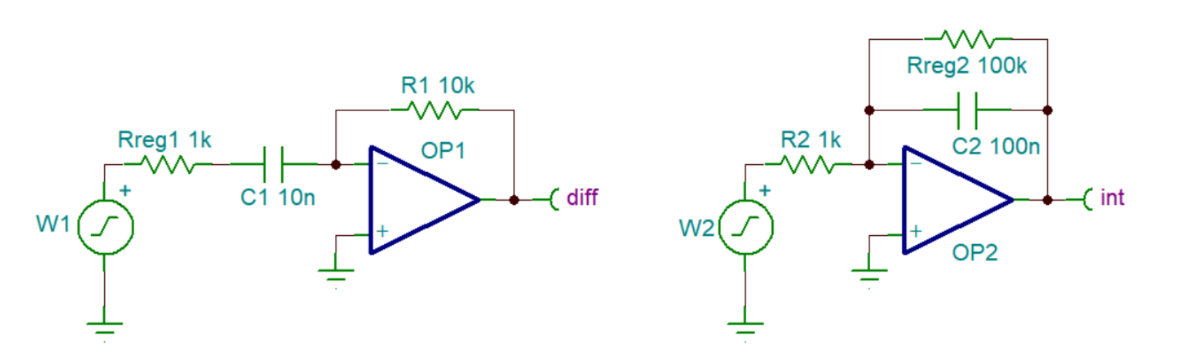
\includegraphics[width=0.9\textwidth]{schema_integratore_derivatore.png}
    }{%
        \fbox{\parbox{0.36\textwidth}{\centering \scriptsize [Circuito Integratore]}}
    }
    
    \vspace{6mm}
    
    {\usebeamerfont{title}\color{TDblue}\Large\textbf{S05 -- Circuiti con OpAmp: Derivatore e Integratore}\par}
    \vspace{3mm}
    
    {\usebeamerfont{subtitle}\normalsize
        Modelli teorici, simulazioni, misure e implicazioni pratiche\par}
    
    \vspace{8mm}
    
    {\usebeamerfont{author}\small
        Alessia Di Nino, Marco Malucchi\par}
    \vspace{1mm}
    {\usebeamerfont{institute}\footnotesize\textbf{Tavolo 10}\par}
    \vfill
\end{frame}

\begin{frame}{Roadmap}
    \tableofcontents[hideallsubsections]
\end{frame}

% ===================================================
\section{Obiettivi \& Setup}
% ===================================================
\begin{frame}{Obiettivi dell'esercitazione}
    \begin{columns}[c,onlytextwidth]
        \begin{column}{0.5\textwidth}
            \centering
            \textbf{\large Focus dell'esperienza}\\[3mm]
            Analisi del comportamento \textbf{ideale} vs \textbf{reale} di integratori e derivatori basati su OpAmp.
        \end{column}
        \begin{column}{0.45\textwidth}
            \begin{block}{Punti chiave}
                \begin{itemize}
                    \item Funzioni di trasferimento $H(\omega)$.
                    \item Risposta nel tempo e frequenza.
                    \item Effetti di saturazione e risonanza.
                    \item Ruolo delle resistenze $R_{\text{reg}}$.
                \end{itemize}
            \end{block}
        \end{column}
    \end{columns}
\end{frame}

\begin{frame}{Schemi circuitali}
    \begin{columns}[T,onlytextwidth]
        \begin{column}{0.48\textwidth}
            \centering
            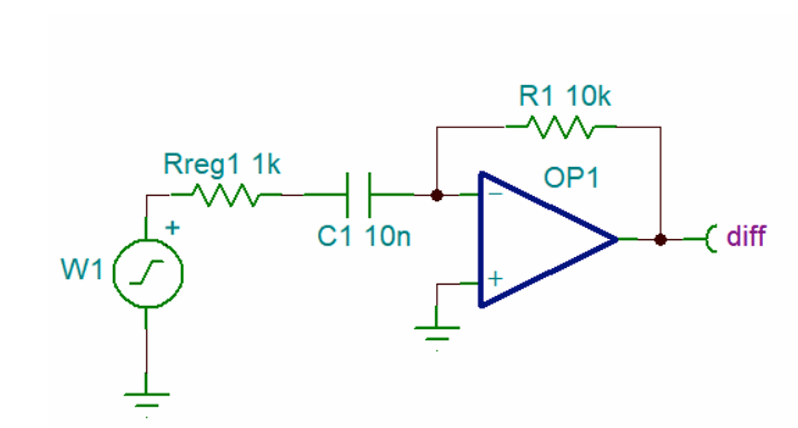
\includegraphics[width=\linewidth]{schema_derivatore.png}
            \caption*{\scriptsize \textit{Schema circuitale derivatore}}
        \end{column}
        \begin{column}{0.48\textwidth}
            \centering
            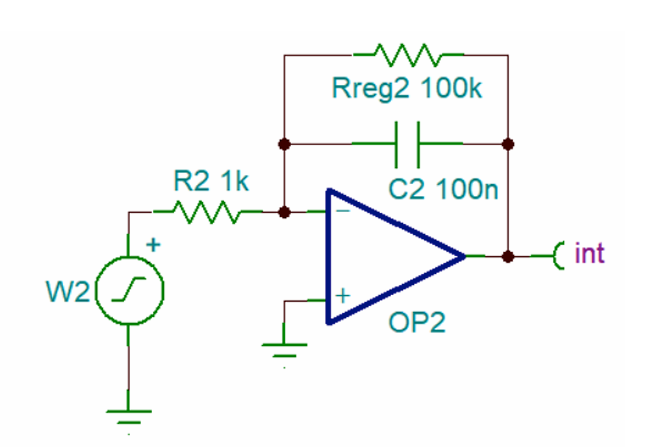
\includegraphics[width=\linewidth]{schema_integratore.png}
            \caption*{\scriptsize \textit{Schema circuitale integratore}}
        \end{column}
    \end{columns}
\end{frame}

% ===================================================
\section{Modelli teorici}
% ===================================================
\begin{frame}{Integratore: Modello Matematico}
    \centering
    \textbf{Integratore ideale} ($A\to\infty$):
    \cleanbox{}{
        \begin{equation*}
        H(\omega)=-\frac{1}{j\omega RC}, \quad V_{\text{out}}(t)=-\frac{1}{RC}\int V_{\text{in}}(t)\,dt
        \end{equation*}
    }
    \vspace{4mm}
    \uncover<2->{
        \textbf{Con resistenza di feedback $R_{\text{reg}}$:}
        \begin{equation*}
        H(\omega)=\frac{R_{\text{reg}}/R}{1+j\omega R_{\text{reg}}C}
        \end{equation*}
        \textit{Osservazione: per $\omega \gg 1/(R_{\text{reg}}C)$ il circuito torna a integrare correttamente.}
    }
\end{frame}

\begin{frame}{Derivatore e Polo Dominante}
    \begin{columns}[c,onlytextwidth]
        \begin{column}{0.45\textwidth}
            \textbf{Derivatore ideale:}\\
            $H(\omega)=-j\omega RC$\\[4mm]
            \textbf{Modello Reale:}\\
            Considerando il guadagno open-loop con polo dominante:
            $$A(\omega)=\frac{A_0}{1+j\omega\tau_{PD}}$$
        \end{column}
        \begin{column}{0.5\textwidth}
            \begin{block}{Stabilità}
                L'assenza di $R_{\text{reg}}$ porta a una marcata \textbf{risonanza} e instabilità ad alte frequenze dovuta al rumore e al limite di banda dell'OpAmp.
            \end{block}
        \end{column}
    \end{columns}
\end{frame}

% ===================================================
\section{Analisi Sperimentale}
% ===================================================
\begin{frame}{Integratore: Risposta Temporale e Frequenza}
    \begin{columns}[T]
        \begin{column}{0.6\textwidth}
            \centering
            \only<1>{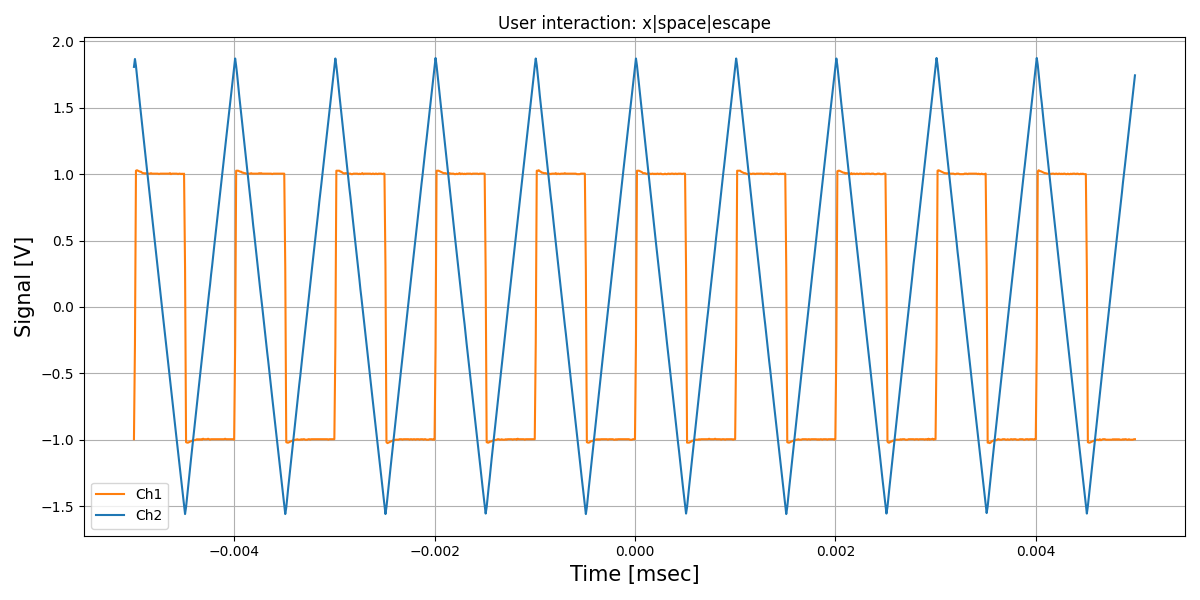
\includegraphics[width=\textwidth]{integratore_1kHz.png}}
            \only<2>{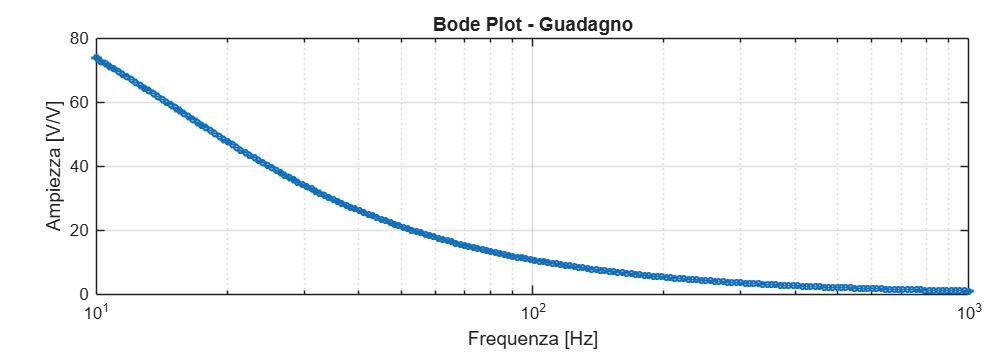
\includegraphics[width=\textwidth]{guadagno_integratore.png}}
            \caption*{\scriptsize 
                \only<1>{Dominio del tempo ($1\,\text{kHz}$): uscita triangolare}
                \only<2>{Risposta in frequenza: attenuazione dei poli}}
        \end{column}
        \begin{column}{0.38\textwidth}
            \vspace{1cm}
            \begin{itemize}
                \item Ingresso quadra $\rightarrow$ Uscita triangolare.
                \item $R_{\text{reg}}$ introduce un guadagno statico finito.
                \item Prevenzione della saturazione DC.
            \end{itemize}
        \end{column}
    \end{columns}
\end{frame}

\begin{frame}{Derivatore: Risposta Temporale e Risonanza}
    \begin{columns}[T]
        \begin{column}{0.6\textwidth}
            \centering
            \only<1>{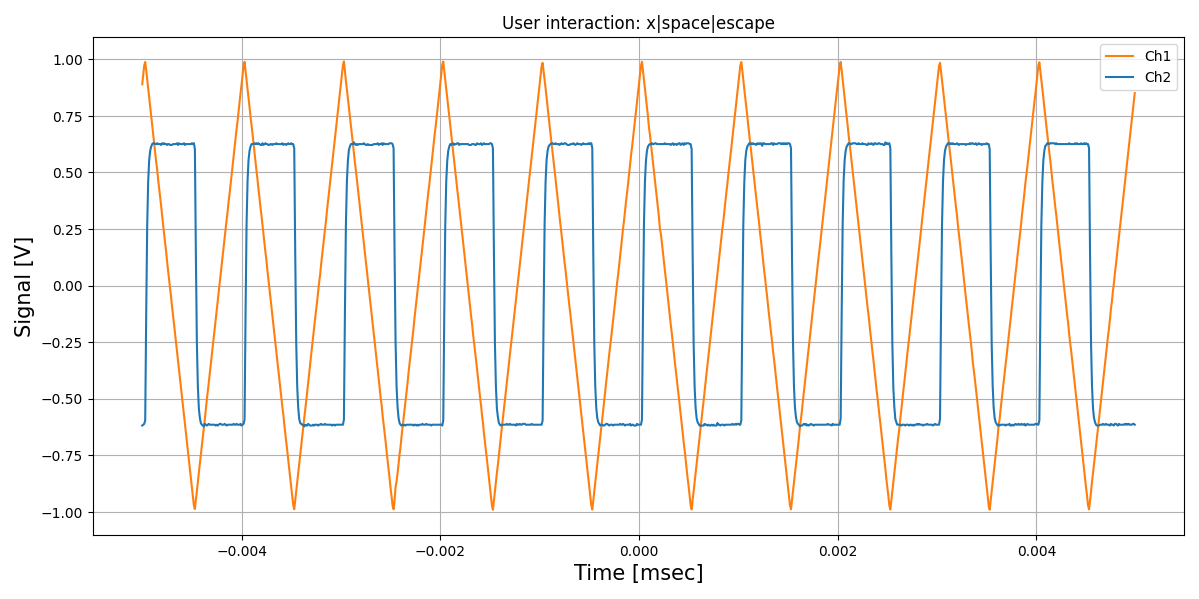
\includegraphics[width=\textwidth]{derivatore_triangle_1kHz.png}}
            \only<2>{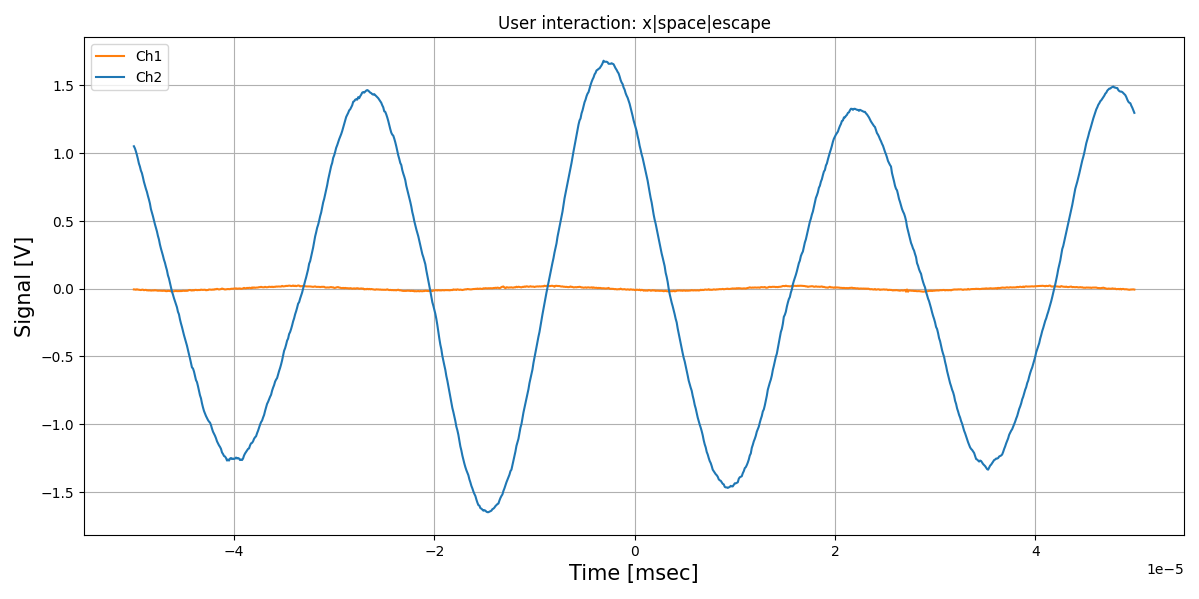
\includegraphics[width=\textwidth]{risonanza_triangle_40kHz.png}}
            \only<3>{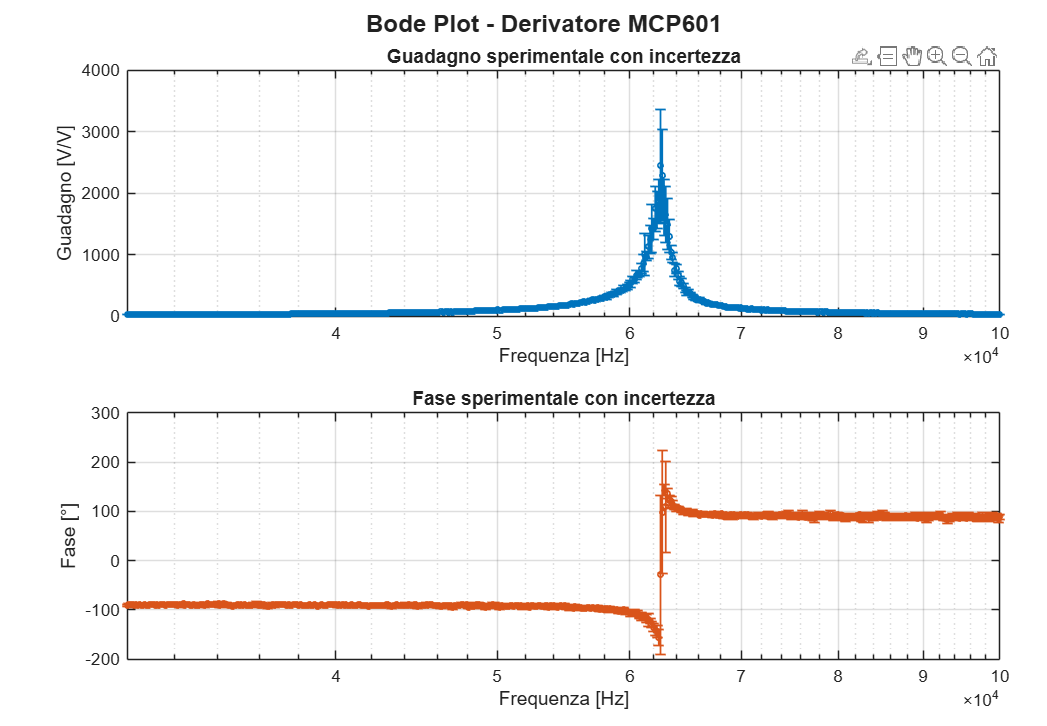
\includegraphics[width=\textwidth]{bode_derivatore.png}}
            \caption*{\scriptsize 
                \only<1>{Derivazione corretta con $R_{\text{reg}}$}
                \only<2>{Effetto di risonanza senza $R_{\text{reg}}$}
                \only<3>{Diagramma di Bode: pendenza $\approx -20\,\text{dB/dec}$}}
        \end{column}
        \begin{column}{0.38\textwidth}
            \vspace{1cm}
            \begin{itemize}
                \item Ingresso triangolare $\rightarrow$ Uscita quadra.
                \item Senza $R_{\text{reg}}$ si osservano oscillazioni (ringing).
                \item Limite superiore imposto dal GBWP dell'OpAmp.
            \end{itemize}
        \end{column}
    \end{columns}
\end{frame}

% ===================================================
\section{Risultati e Conclusioni}
% ===================================================
\begin{frame}{Bode a confronto: l'effetto di $R_{\text{reg}}$}
    \centering
    \begin{columns}[onlytextwidth]
        \begin{column}{0.48\textwidth}
            \centering \textbf{Integratore}
            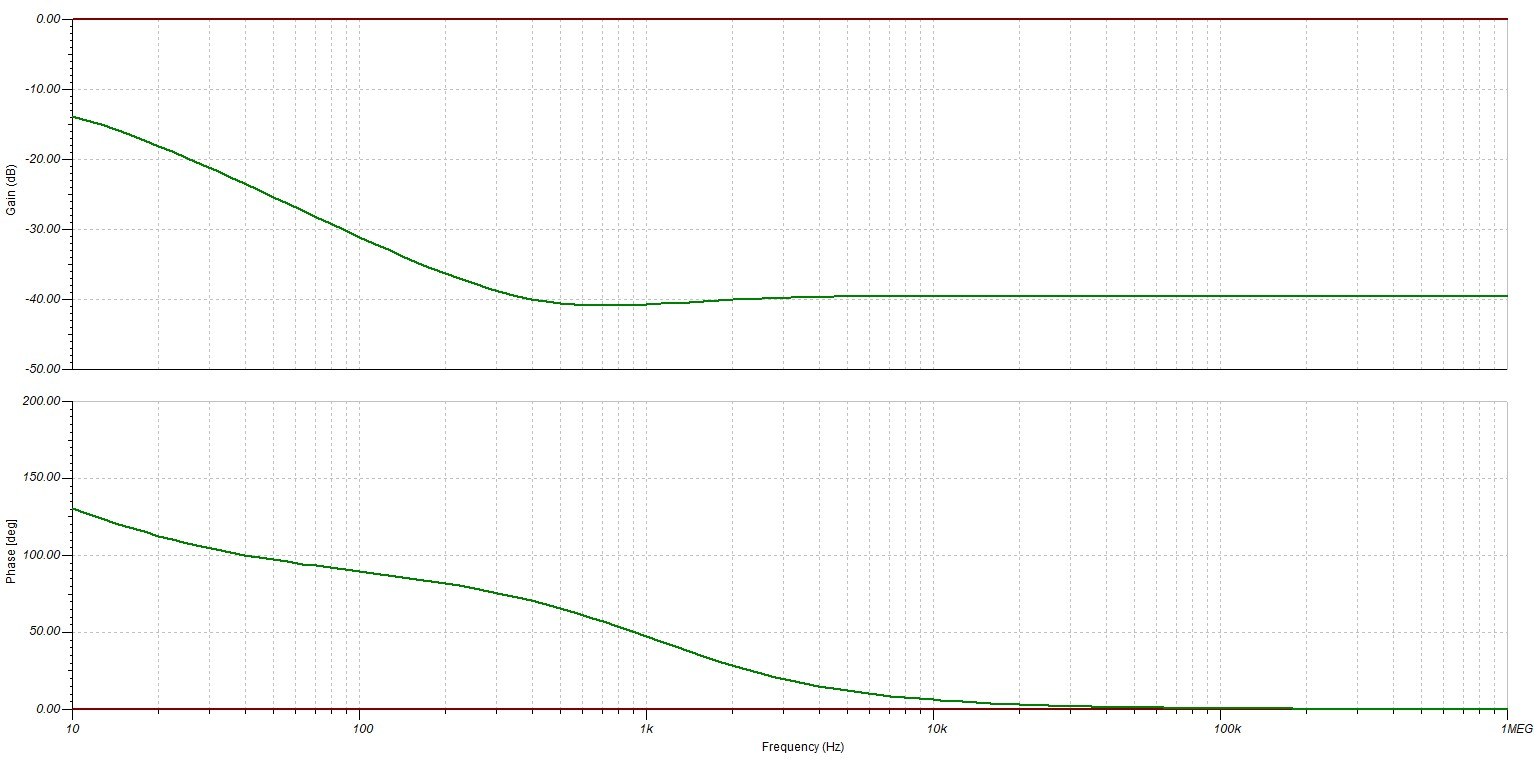
\includegraphics[width=0.8\linewidth]{tina_integratore_sweep.jpg}
            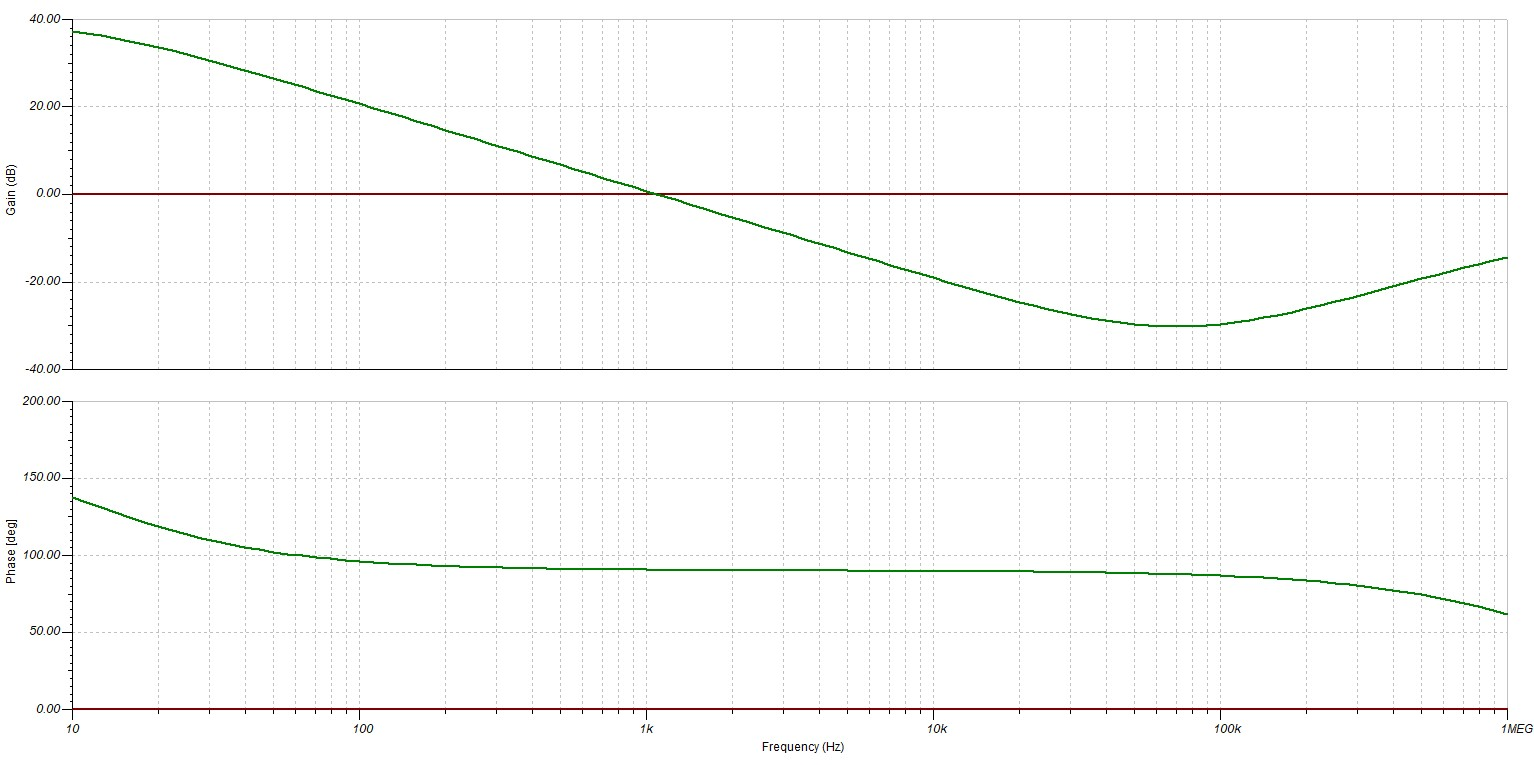
\includegraphics[width=0.8\linewidth]{tina_integratore_sweep_reg.jpg}
        \end{column}
        \begin{column}{0.48\textwidth}
            \centering \textbf{Derivatore}
            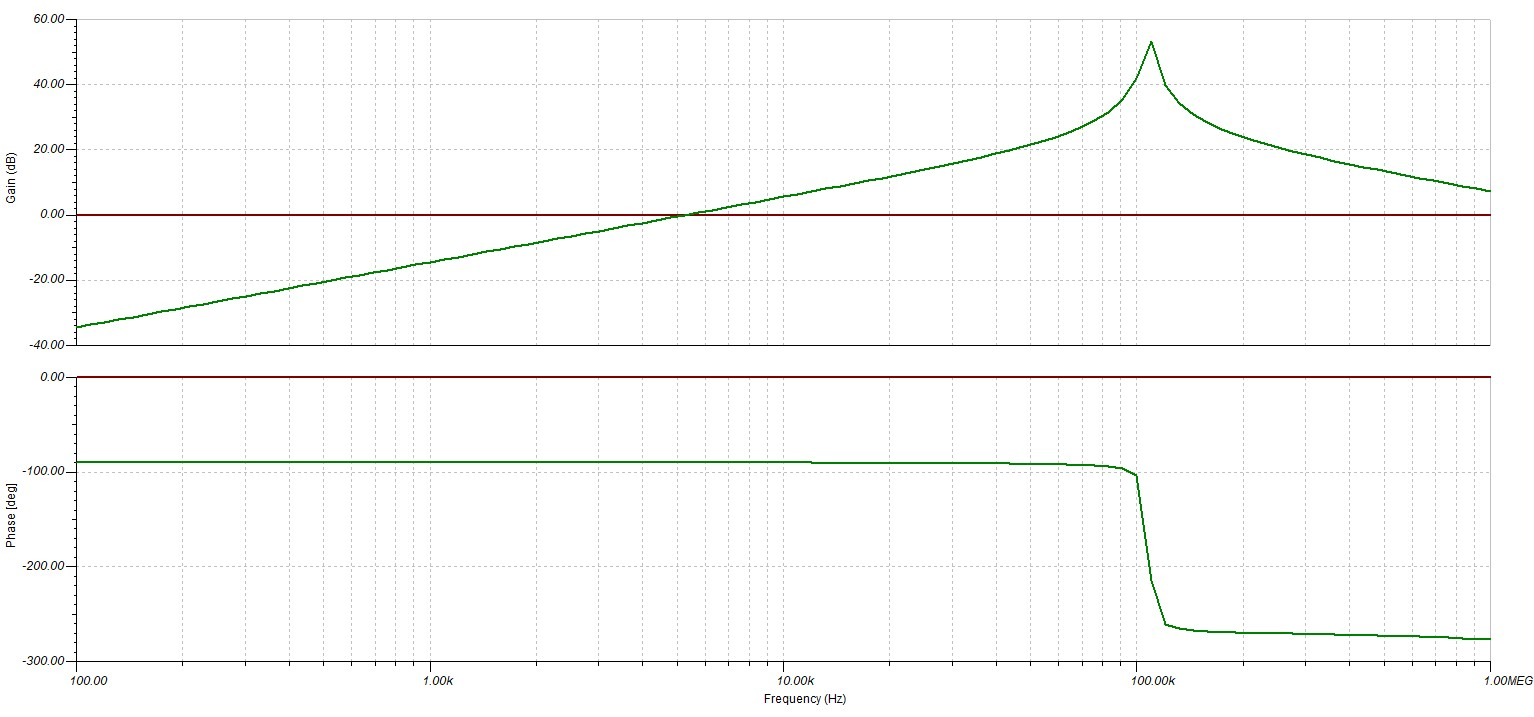
\includegraphics[width=0.8\linewidth]{tina_derivatore_sweep_c=15n_R=2k.jpg}
            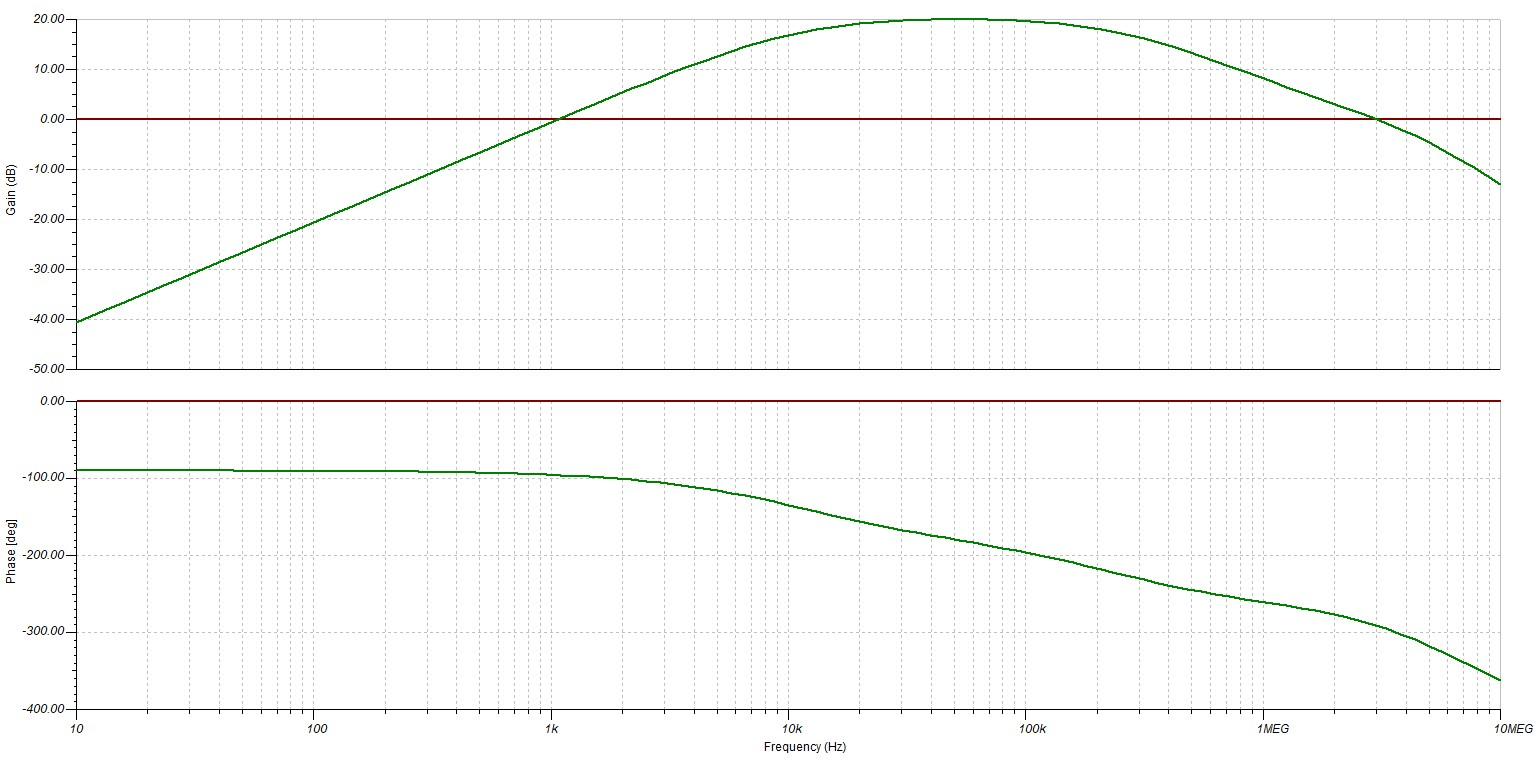
\includegraphics[width=0.8\linewidth]{tina_derivatore_sweep_reg.jpg}
        \end{column}
    \end{columns}
    \vspace{2mm}
    \cleanbox{}{\scriptsize \textbf{Takeaway:} $R_{\text{reg}}$ limita il guadagno a bassa $f$ per l’integratore e smorza la risonanza del derivatore.}
\end{frame}

\begin{frame}{Conclusioni e Takeaway}
    \begin{columns}[c]
        \begin{column}{0.6\textwidth}
            \begin{itemize}
                \item \textbf{Stabilità}: $R_{\text{reg}}$ rende i circuiti fisicamente realizzabili.
                \item \textbf{Offset}: $V_{\text{off}}$ è critico per l'integratore (accumulo).
                \item \textbf{Banda}: Il modello ideale vale solo tra $f_{\text{low}}$ e $f_{\text{high}}$ definite dai componenti di regolazione e dal GBWP.
            \end{itemize}
        \end{column}
        \begin{column}{0.35\textwidth}
            \centering
            \begin{table}
                \scriptsize
                \begin{tabular}{|l|c|}
                    \hline
                    \rowcolor{TDlight} \textbf{Problema} & \textbf{Soluzione} \\ \hline
                    Saturazione Integr. & $R_{\text{reg}}$ Feedback \\ \hline
                    Risonanza Deriv. & $R_{\text{reg}}$ Ingresso \\ \hline
                    Rumore Alta $f$ & Filtro passa-basso \\ \hline
                \end{tabular}
            \end{table}
        \end{column}
    \end{columns}
\end{frame}

\begin{frame}[plain]
    \centering
    \vspace{2cm}
    {\color{TDblue}\Huge \textbf{Grazie per l'attenzione!}}
    \vspace{1cm}
    \par Alessia Di Nino, Marco Malucchi -- Tavolo 10
\end{frame}

\end{document}